%\documentstyle[astro,psfig]{article}
\documentclass{article}
\usepackage{psfig}
\usepackage{astro}
\usepackage{times}
\GoodMargins
\newcommand{\note}[1]{({\bf #1})}
\title{Variability Pipeline}
\author{Eugene Magnier}
\begin{document}
\maketitle

\section{Overview}

The Loneos Pipeline provides automated reduction of images, including
photometry and astrometry, with the final data stored in a photometry
database organized by star position on the sky.

Fig.~\ref{pipeline} shows a schematic of the analysis pipeline.
Images are written to the disk from the camera by the software which
runs it, {\tt astrocam}.  The resulting images are FITS files (which
may be arbitrarily sized) and have header keyword parameters RA and
DEC specifying rough celestial coordinates.  Images are first analyzed
by {\tt dophot}, which produces instrumental photometry and pixel
coordinate positions for stars and other objects in the images,
writing files with a particular format, called OBJ files in this
discussion.  The results from {\tt dophot} are cleaned up by a program
called {\tt fstat} which merges the header information from the image
with the most relevant parts of the OBJ file, creating a new file with
the CMP format.  Astrometry is performed on the CMP file with the
program {\tt gastro}.  {\tt Gastro} makes a comparison with an
astrometric reference database and only changes CMP header keywords as
a result.  Finally, the processed image CMP file is added to the
photometry database with the program {\tt addstar}.  The photometry
database is maintained in a large number of files (CPT files), each
representing a small region of sky.  There is no relationship between
the image locations and the boundaries of CPT file.  All of these
processes occur on individual image, and would typically be performed
while the observations are occuring, or during the day following, but
may be performed at any time to add new or archived data to the
database.

Once large batches of images have been processed, a series of programs
should be run to clean up the photometry database.  Typically, these
routines would be run at the end of a night on all of the CPT files to
which new data were added.  First, {\tt markstar} identifies bad data
(the trails of satelites, the bleeding columns from stars, ghost
images), and flags these data points appropriately.  Second, {\tt
  addusno} matches the catalog stars with stars from the USNO database
and adds the USNO magnitudes to the photometry database.  Next, {\tt
  markrock} searches for likely asteroids in the CPT file, marks them,
and writes the asteroid observations to an asteroid database.  It also
notes measurements which are likely to be noise and cosmic rays.
Finally, {\tt nrphot} determines relative photometric calibrations for
observations in a set of CPT files.  

With the exception of {\tt dophot}, all of the programs in the
pipeline refer to a single configuration file to determine the large
number of parameters necessary in the process.  The default parameter
file is hardwired into the programs, but an alternate configuration
file may be specified with the environment variable {\tt
  PIPE\_CONFIG}.  This option makes independent processing of multiple
data sources trivial.  For example, if the pipeline is to be used for
both Loneos and SDSS image analysis and display, there could be two
configuration files (eg, {\tt loneos.txt} and {\tt sdss.txt}), one for
each data source.  Several important parameters would be different
between these two, for example, the initial plate scale guess for the
astrometry routine, or the parameters which define the rough chip
orientation.  This scheme allows for analysis of different types of
images, with a common destination photometry database, or for
independent photometry databases.

\begin{figure}
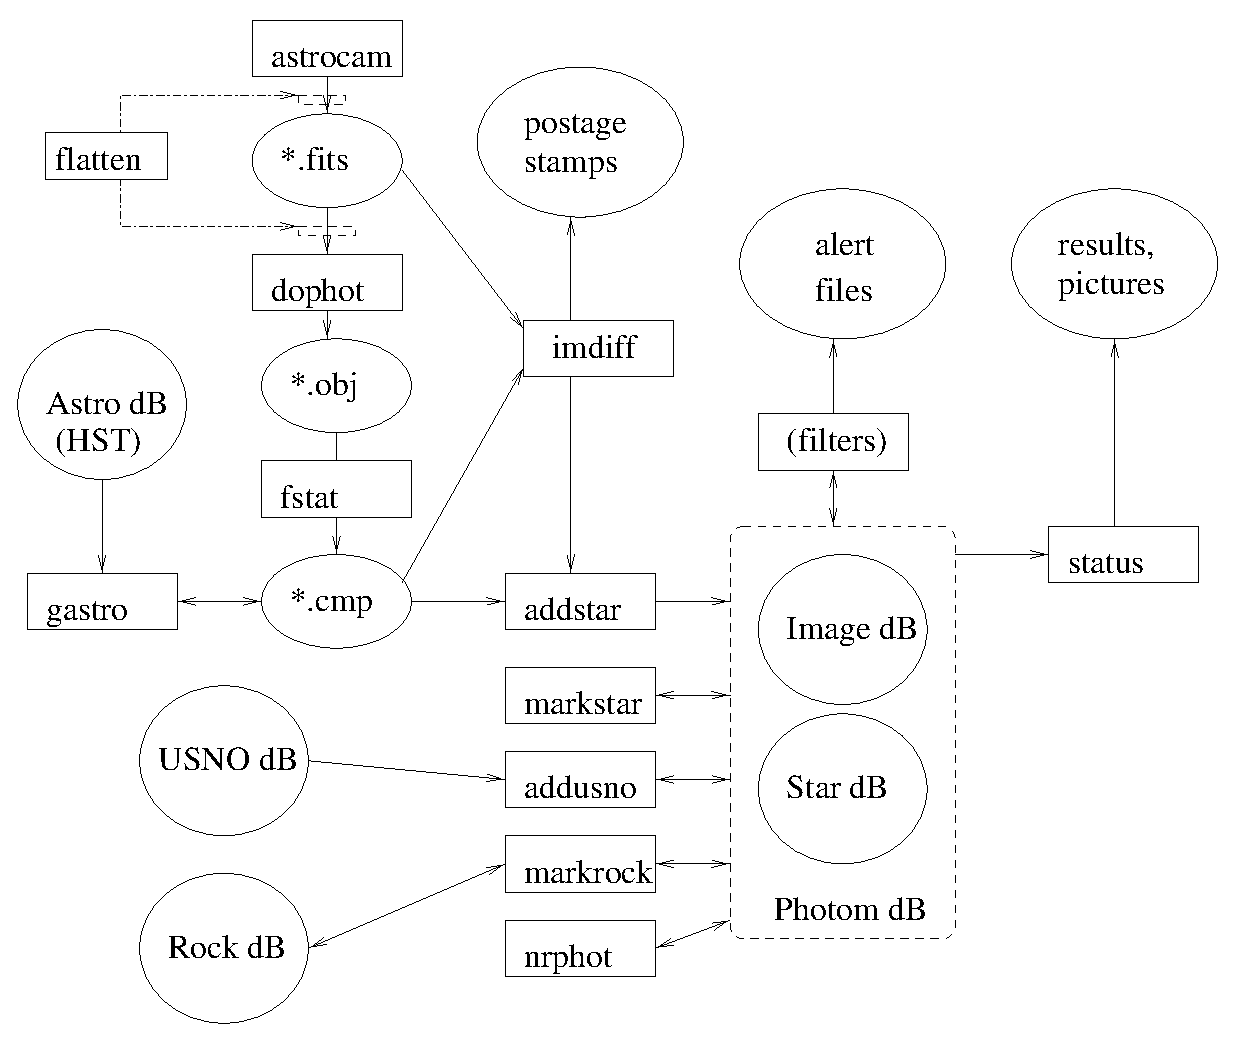
\psfig{file=schematic.eps,width=9cm}
\caption{\label{pipeline} 
Schematic of the photometry pipeline.  Rectangles represent programs,
while ovals represent data products.  Arrows show the direction of
travel of information.  The flatten routine is a filter whose position
may change as the pipeline matures.
}
\end{figure}

Data from different sources can be processed by the pipeline and
stored in the same photometry database, since all photometry is tagged
with a source ID in the database (as are the images in the image
database).  This allows us to include, for example, the USNO catalog
magnitude measurements (or a subset) in the photometry database for a
quick comparion.  Different sources may be considered different
filters, so color-color and color-magnitude diagrams could be
extracted by specifying choices for source catalog.  Currently each
object has a single primary photometric system, and individual
observations may be combined to determine that average (eg, if they
are different photometry sources with roughly the filter bandpass) or
they may be ignored when calculating relative magnitudes (eg, the USNO
magnitudes would be ignored).  This may be expanded upon by defining
multiple average magnitudes and allowing different measurements to
contribute only to the appropriate average.  The determination of the
photometry code for a particular image is currently not well defined.
There are several points in the analysis where the user (or the
controlling program) may specify the photometry source.  A table
should be kept in the photometry catalog to define the various
photometry codes.  

\section{Image Analysis Pipeline}
\label{parallel}
\subsection{Photometry -- Dophot}

Photometry is performed using a varient of {\tt Dophot}.  The version
of dophot is based on Dophot 2.0, but it has been adapted to
streamline processing of many files.  First, with this version of
dophot, any FITS format data is safely read in.  Instead of compiling
to a fixed maximum size, only the memory needed to contain the image
matrix is allocated.  The image is also converted to REAL*32 from
whatever BITPIX for processing.  Finally, only a single, complete
parameter file is loaded by dophot.  There is no option for a modified
and a default parameter file.  The parameter file to be used is
defined, along with the input image and the output object list on the
command line when the program is run: \\
{\tt dophot image.fits image.obj parameter\_file} \\
To achive this, the code from dophot was wrapped within a C program
which interprets the command line arguments, allocates the necessary
memory, and reads in the image.  The rest of the processing is
performed by dophot in the standad manner.  Notice that we use a
consistent naming convention through the pipeline reductions.  The
image is called {\tt foo.fits}, while the resulting dophot-produced
photometry list is called {\tt foo.obj}.  

\subsection{Cleanup -- fstat}

After an image is processed by dophot, the object file ({\tt foo.obj})
is converted to a more-compact, more-complete file called a CMP file,
with a name of the form ({\tt foo.cmp}).  This conversion is done with
the program {\tt fstat}.  The CMP file consists of the FITS header
from the original image ({\tt foo.fits}), with some additional
keywords to be used at later stages in the analysis, followed by an
ASCII list of the interesting data from ({\tt foo.obj}).  In this
list, types 6 and 8 are excluded, and only the following values are
kept:
\begin{verbatim}
X       Y     Mag   dMag t log(sky) 
1342.0  106.1 14.166 000 4 3.2
\end{verbatim}
Objects with a signal-to-noise ratio lower than a specified cutoff
({\tt MIN\_SN\_FSTAT}) are also excluded.  Some general information
about the image is derived by {\tt fstat} (FWHM, saturation and
completeness limits, number of each dophot type) and stored as
keywords in the header.  The photometry source must be specified at
this stage as one of the command line arguments, though the value used
may be overridden in one of the stages belowe.  The resulting file can
now stand on its own without reference to the original image.  The
keywords used by {\tt fstat} include the minimum signal to noise, a
rough guess at the zero point ({\tt ZERO\_PT}), and four numbers
defining the format of the {\tt dophot} OBJ file.

\subsection{Astrometry -- gastro}

Astrometry is performed automatically by the program {\tt gastro}.
{\tt gastro} loads a CMP file and determines an initial guess for the
center coordinates (based on the RA and DEC header keywords).  The
program also uses the configuration information about the plate scale
and rough orientation of the image to get a close to the final
solution.  Also, the true sky position of the telescope pole may be
defined to allow astrometry on images taken close to the pole.  The
comparison is made with the astrometric catalog, which may be the HST
Guide Star Catalog, or it may be any source if the data is placed in
the correct format.

\section{The Photometry Database}

\subsection{Photometry File Format}
The photometry database consists of a large number of photometry files
representing sections of the sky and a file containing information on
the images incorporated in the database.  These files are called
alternatively ``region files'' or CPT files (because they have the
extension {\tt .cpt}).  The photometry files are sorted by Declination
into different directories, each consisting of a band 7.5\degree\ 
wide.  These directories have names like n0730, representing the band
starting at a Declination of +07:30.  The image database (Images.dat)
is stored in the upper level directory of this directory tree.  In
fact, the locations of the Images.dat file, the photometry database,
and such are all flexible and may be changed by altering the
configuration file.

The name and location of each sky region comes from the Hubble Space
Telescope Guide Star Catalog.  There is a file, GSCregions.tbl, which
can be used to find the region file appropriate for any location on
the sky.  A number of routines exist to make such a query.  

Each photometry file in the photometry database contains all
observations and all average values for all stars observed within the
appropriate region on the sky.  The identity of stars is essentially
determined by the RA and DEC coordinates.  In very crowded regions,
the end user may need to double check that a neighboring star is not
contaminating individual detections (see the discusion on {\tt
  addstar} below).

The photometry files are stored in a binary format, both to reduce the
volume and to speed access.  As a result, the interpretation of the
data is machine dependent: little endian machines need to swap the
data intelligently.  Fortunately, this operation is taken care of
appropriately, if the programs are compiled with the BYTESWAP option
set as needed, which is automatically set by the Makefile in the case
of a Linux machine.  For reference, Suns, SGI, and HP are all big
endian, while PCs and DECs are little endian.  The automatic
conversion takes place by using the funcions {\tt Fread} and {\tt Fwrite}
to substitute for the standard C library {\tt fread} and {\tt fwrite}
functions.  {\tt Fread} and {\tt Fwrite} are told the datatype being read,
and they know the layout of the bytes for a particular datatype.
Anytime the definitions of the relevant structures (see below) are
changed, {\tt Fread} and {\tt Fwrite} must be updated.  Fortunately, there
is only one file ({\tt Fread.c}), and it has a single byteswapping
section, making it easy to adjust the code appropriately.

The format of a single photometry database file consists four
sections:  
\begin{itemize}
\item {\bf header} -- this is a standard FITS header with room for comments
  about the file or whatever.  Since the rest of the file is not a
  standard FITS file, the SIMPLE keyword is set to False.  The three
  necessary keywords are NSTARS, NMEAS, and NMISS, which define the
  sizes of the next three sections.
\item {\bf average} -- this section contains all average measurement
  quantities for each star in the file.  There are NSTARS entries, and
  each entry is the data from a structure of type Average (defined in
  loneos.h, and discussed in more detail below).  Thus, the total size
  in bytes of this section can be found by NSTARS*sizeof(Average).
\item {\bf measure} -- this section contains the individual
  measurements for each star in the database.  There are NMEAS
  entries, and like the average section, each entry is a single
  structure, in this case of type Measure (in loneos.h, see below).
  All measurements of a single star are consecutive.  The number of
  measurements for a single star is defined by average.Nm and the
  starting entry for a single star is given by average.offset.
  Therefore, the first measurement of a specific star average[500]
  would be given by measure[average[500].offset], while the second is 
  measure[average[500].offset + 1], and so forth.  
\item {\bf missing} -- this section contains references to all missing
  measurements of a star.  This means all of those occasions when an
  image enclosed the location of a star in the database, but no star
  was detected on the image.  Similar to the case of the measure
  section, each star has a number of missing entries (which may be 0)
  given by average.Nn, and the first missing entry is given by
  average.missing.  Each missing entry value is again a structure of
  type Missing.  Currently, the only data in the structure is the time
  of the observation, which allows for an unambiguous recovery of the
  image where the star was missed.
\end{itemize}

\subsubsection*{Average Structure defined in loneos.h}
\begin{verbatim}
typedef struct {
  float R;                    /* RA  in decimal degrees */
  float D;                    /* DEC in decimal degrees */
  short int M;                /* thousandths of mag (-32.000 to 32.000 valid range) */
  unsigned short int Nm, Nn;  /* number of measurements, missing */
  short int Xp, Xm;           /* log(chisq) values in tenths */
  unsigned short int code;    /* an ID code (ie, star, ghost, satelite, etc) */
  signed int offset;          /* offset to first measurement */
  signed int missing;         /* offset to first missing obs */
} Average; /* 28 bytes / Average */
\end{verbatim}
The structure above defines the average data stored in the photometry
database for each star.  Most of the entries are self-explantory, but
some need a bit of clarification.  The two $\chi^2$ entries ({\tt Xp}
and {\tt Xm}) are the $\chi^2$ values of the average position and the
average magnitude.  These are stored as logarthmic quantities because
high dynamic range is not needed.  For the magnitude, the assumption
is that the star brightness is constant and the $\chi^2$ incorporates
the photometric errors on each measurement.  For the postion, the
a default constant error is used \note{True?} and again the assumption
is that the postion is constant.  As discussed above, the values of
{\tt Nm} and {\tt Nn} give the number of measurements and missing
observations for this star, while the entries {\tt offset} and {\tt
  missing} point to the first {\bf measure} and {\bf missing} entry
for this star.  The entry {\tt M} is the current best average
magnitude solution for this star (see the section on Relative
Photometry).  Finally, the entry {\tt code} is an ID code for each
object, which may define a variety of things about the object.  For
example, if the object is known to be variable, or if the object is
associated with a USNO star, or if the object is a measurement of an
asteroid.  See below for details of these definitions.

\subsubsection*{Measure Structure defined in loneos.h}
{\small
\begin{verbatim}
typedef struct {
  short int dR, dD;           /* 1/100 of arcsec (-327.67 to +327.67 valid range) */
  short int M;                /* thousandths of mag (-32.767 to 32.767 valid range) */
  short int Mcal;             /* image cal mag, thousandths of mag (-32.767 to 32.767 valid range) */
  unsigned char dM;           /* thousandths of mag (0.000 to 0.255 valid range) */
  char dophot;                /* dophot type (1-9) */
  unsigned short int source;  /* code to identify photometry source */
  unsigned int   t;           /* time in seconds (0 - 143 years valid range) */
  unsigned int average;       /* reference to corresponding average entry */
  /* upper byte of Measure.average stores flags:
   limit of 16,777,215 stars (Naverage) in a file (=0xFFFFFF) 
   flags: average & 0x1000000 */
} Measure; /* 20 bytes / Measure */
\end{verbatim}
}
The structure above defines the individual measurement data stored for
each observation of each star.  The first two entries, dR and dD, are
the difference between the average coordinates for this star and the
coordinates determined for this observation.  Clearly, if this
residual is too large, the individual measurement will not be
successfully matched with the average star position.  {\tt M} and {\tt
  dM} are the instrumental magnitude and error for this measurement,
after correction for the exposure time and a zero point (defined in
the configuration file as ZERO\_PT).  The entry {\tt t} determines the
time of the individual observation.  This is important not only for
timing purposes, but also to determine the source image for this
observation.  The time and the entry {\tt source} uniquely determine
the image in the image database that generated this measurement.
Furthermore, this correspondence allows for determination of the pixel
coordinates on the chip, by going throught the image astrometry stored
in the Image database (see below).  The entry {\tt source} is a code which
identifies the particular CCD/Telescope/Filter setup.  Each unique
{\tt source} should be treated as an independent filter set for the
purposes of accurate relative photometric comparisons.  This entry
also allows external catalog data, such as the USNO or Sloan
photometry, to be added to the database, as desired.  The entry {\tt
  average} is a pointer back to the {\bf average} section to allow
determination of the star from the measurements, in addition to the
reverse.  The bits of the upper byte of this value are reserved for
flags used to define particular situations for this measurement.
Possible values are:
\begin{itemize}
\item 1 = BLEND\_IMAGE - the star on the image matched more than one
  catalog star
\item 2 = BLEND\_CATALOG - the star in the catalog matched more than
  one image star
\item 4 = UPPER\_LIMIT - \note{not really used?}
\item 8 = CALIBRATED - relative photometry has been performed at least
  once.
\end{itemize}
The entry {\tt dophot} stores the dophot type for this particular
measurement (1-9: four extra bits in this field).   
Finally, the value {\tt Mcal} determines the photometric calibration
of this specific measurment.  This value is an offset appropriate to
this image (and if needed, this point in time and this chip position)
to bring the observations of the stars on multiple images to a common
system (see the section on relative photometry).

\subsection{Image Database}

All images for which photometry has been included in the photometry
database also have entries in an image database.  The image database
is (currently) a single file in the upper directory of the photometry
database.  The name of the file is determined by the IMAGE\_CATALOG
entry in the configuration file, and is currently set to Images.dat.
Like the photometry database files, the image database consists of a
FITS header followed by binary data.  There is only one type of binary
data: each image has an entry, which is the data from a structure of
type Image (loneos.h).  The number of images in the file is determined
by the {\tt NIMAGES} keyword.  If the number of images becomes too
large, extrapolation of the system to a set of image database files
with a reference list is quite straightforeward, and could be modeled
on the organization of the region files (eg, one image database file
for each Declination directory).

\subsubsection*{Image Structure defined in loneos.h}
{\small
\begin{verbatim}
typedef struct {
  Coords         coords;            /* 120 bytes */
  unsigned int   tzero;             /* readout time row 0 in sec (0 - 142 years valid range) */
  unsigned int   nstar;             /* number of stars on image */
  short int      secz;              /* thousanths of airmass (valid range -32.000 -- 32.000) */
  short int      NX, NY;            /* dimensions of image */
  short int      apmifit, dapmifit; /* aperture correction and error in thousandths of mag */
  short int      source;            /* identifier for CCD (each ever used will have a unique letter) */
  short int      Mcal;              /* thousandths of mag (-32.000 -- 32.000 valid range) */
  short int      dMcal;             /* thousandths of mag (-32.000 -- 32.000 valid range) */
  short int      Xm;                /* 10*log(image chi-square) */
  char           name[32];          /* name of original image */
  unsigned char  detection_limit;   /* tenths of mag (0.0 - 25.6 valid range) */
  unsigned char  saturation_limit;  /* tenths of mag (0.0 - 25.6 valid range) */
  unsigned char  cerror;            /* astrometric error: 1/50 of arcsec (0 -- 5.12 valid range) */
  unsigned char  fwhm_x, fwhm_y;    /* PSF terms in 25*arcsec (valid range 0.0 -- 10.2" ") */
  unsigned char  trate;             /* 10000 * scan rate in sec/pix (0 -- 0.0256 valid range, 
                                       typically 0.0146. this is used only to determine the time
                                       of the observation, not to find the coordinates.  1 byte
                                       gives 0.11 sec accuracy */
  char           code;              /* flag to mark an image as bad or whatever */
  char           dummy[7];          /* extra space for the future?  (seems like a lot!) */
  float          exptime;           /* exposure time, seconds */
} Image;  /* 192 bytes / Image */
\end{verbatim}}
The structure above lists all of the data stored for each image.  A
substantial amount of information is stored for each image.  First,
the astrometric calibration information is stored in a {\tt Coords}
structure (see coordinate systems, above).  The upper and lower limits
of the photometry in the database (in instrumental magnitudes) is
stored in {\tt detection\_limit} and {\tt saturation\_limit}.  These
values are useful for comparison for those stars where observations
are missing.  The relationship between time and pixel coordinates is
given by {\tt tzero} and {\tt trate}.  Drift images will have a scan
rate stored in {\tt trate}, while staring images will have a value of
0.0 for this entry ({\tt tzero} then applies to the whole image).
Other important parameters are kept: the astrometric error ({\tt
  cerror}), the airmass ({\tt secz}), the exposure time ({\tt
  exptime}), the number of stars detected ({\tt nstar}), the FWHM
values ({\tt fwhm\_x, fwhm\_y}), the image name ({\tt name}), and the
size of the image ({\tt NX, NY}).  The entry {\tt source} is used as
above to define the CCD/Telescope/Filter used for this observation.
The entry {\tt code} is used to flag images in various ways.
Currently, only one bit is used, to define if the image has
unacceptable photometric scatter.  Seven extra bytes are stored for
future additions.

\subsection{Data Incorporation -- {\tt addstar}}

Images which are completely processed ({\tt dophot, fstat, gastro}) are
then incorporated into the photometry database with the program {\tt 
addstar}.  This program decides which region files are appropriate
for this particular image, then one-by-one adds stars from the image
to the appropriate region file.  Stars already in the catalog are
matched with stars in the new image purely by a positional comparison.
In order to avoid the difficulty of comparisons in the RA and DEC
coordinate frame, a cartesian projection is performed.  The stars from
the image being processed and the database stars in the same area are
projected onto a tangent plane and positional comparisons made in this
(locally cartesian) coordinate frame.  This avoids the dangerous
singularities at the pole and also makes the RA 0,360\degree\ boundary
a trivial problem.  

Several choices must be made in the comparison process.  If a star in
the catalog is matched with a star in the image, the new measurements
of that star are added to the database.  If a star in the database
lies in the field of the image, but is not detected, this information
is added to the list of missing data.  The only data stored in this
case is the time and source, which is sufficient to unambiguously
identify the source image from the image database.  This allows later
programs to find relevant statistics from the image database, if
necessary.  If a star is detected in the image, but is not already in
the database, a new entry is added to the database.  In addition, the
same ``missing data'' from all previous observations images which have
covered this location (ie, images already in the image database) are
included.  This last step is necessary so that the image processing
order is not important.  

Stars also run the danger of being crowded together.  Since all
comparisons are performed on the basis of position alone, crowded
fields may make for ambiguous cross-identifications.  A pair of stars
are matched if the difference in their positions is less than a
specified search radius (usually dependent on the astrometric for the
image).  If more than one catalog stars is correlated with a star in
an image, the new measurement is added to {\em both} catalog stars,
and a flag is set noting that this observation had a blended IMAGE.
Conversely, if a single catalog star is matched with more than one
image star, both new measurements are added to the one catalog star,
and a different flat is set, noting that this observation had a
blended CATALOG.   

\section{Catalog Update and Cleaning}

Occasionally, once a large number of images have been added to the
photometry database, a set of programs should be run to clean and
update the CPT files.  This may best be done on CPT files after a
night's worth of data is incorporated.  These routines define bad
data, identify the USNO catalog stars, and search for asteroids and
other junk.  Most of the results from these routines are the addition
of object flags to the Average data structures (Average.code).  Most
of these routines process data within a single CPT file at a time.

\subsection{Markstar}

The first of the update programs, {\tt markstar}, identifies bad data
and flags it.  It makes three types of identifications: bright stars,
ghost stars, and trails.  In the first case, it searches the HST guide
star catalog for bright stars within the field of the current CPT
file.  Three types of pixels are flagged for bright stars.  Any
measurements within a circular region centered on the star are suspect
(the ``halo'' of the bright star).  Second, points along the X axis
are likely to contain flux from the diffraction spikes.  Finally,
points along the Y axis are likely to have bleeding in addition to the
diffraction spikes.  Each of these three regions has a different size
and range which must be defined in the configuration file.  The
regions are represented by a representative magnitude and a scale
parameter.  For example, the diameter $d$ of the halo for a star with
magnitude $m$ is defined as 
$d = \mbox{BRIGHT\_HALO\_SLOPE} (m - \mbox{BRIGHT\_HALO\_MAG})$.  The X and
Y axis points are defined by the length of the diffraction spike, with
an equivalent formula, and the width of the spike.  Since these are
each independent, there are 8 parameters to define the exclusion
regions of bright stars.  One of the current drawbacks of this system
is the reliance on the HST Guide Star photometry.  In the HST Guide
Star Catalog, only one photometry band is given, so no color
information is available.  The parameters currently used were defined
based on a large number of bright stars, with no adjustment for the
different effective filter system of the Loneos telescope and the HST
GSC.  Thus, occasionally very red stars will be several magnitudes
brighter in the real data than reported in the catalog.  As a result,
large numbers of bad data points in these halos and spikes may be
missed.  

The second type of bad data flagged by {\tt markstar} are the trails
from satelite and other space junk.  This portion of the program
searches for objects which land along a line and which have a high
linear density.  Parameters may be adjusted to define the width and
the necessary density or number of points in the line.  Objects in
lines are also only identified if all observations come from a common
image.  If an object only has one measurement and it is in a trail,
the entire Average is flagged to be bad.  However, if an object has
many measurements and only one is bad, the object is only flagged as
having some bad data points.  

The third type of bad dat are ghost star images.  The HST GSC is
searched for stars projected across the telescope optical axis, which
is defined by the user.  All objects within a region of fixed size is
marked for ghost stars brighter than a specific cutoff magnitude.
Similar to the trails, the average is marked as bad only if all
detections of an object are ghost images.  Otherwise, it is noted that
some data may be bad.

\subsection{Addusno}

The program {\tt addusno} makes two types of identifications of stars
with the USNO catalog.  First, it searches for coincidences within a
small, specified radius.  The choice of this radius is somewhat
tricky: it is important to catch the association, but also to avoid
making too many associations.  Unfortunately, astrometric errors in
the USNO catalog make it necessary to choose a surprisingly large
radius of 5\asec.  To avoid making double matches (matching the two
USNO stars to the same photometry database object), only the USNO
object closest to the object is associated.  There are also a
substantial number of stars with significant proper motion between the
USNO epochs and the current date.  It is not unusual to see 8-15\asec\ 
discrepancy for specific stars.  To catch these objects, any objects
which do not match the USNO database, but which have more than a
minimum number of measurements (2 or 3?) are searched for more distant
USNO companions.  A large, user-specified radius is used for this
search.  Of course, only USNO stars which are not already matched to
the database may be candidates for the proper motion match.  This
stage is suceptible to errors in that a slow-moving solar-system
object may be associated with a faint USNO star.  For this reason,
objects flagged as high proper motion stars should be taken with some
caution.  Of course, during the {\tt addusno} stage, no objects
already flagged as bad by {\tt markstar} will be matched with USNO
stars.  

\subsection{Markrock}

Once stars have been identified with the USNO database, it is possible
to search for asteroid detections.  The program {\tt markrock}
searches within a specific CPT file for objects which are moving along
straight lines in (X,Y,t) space.  In order for an object to be found
by {\tt markrock}, it must have three points, each with only single
measurements.  The third point must land within a specified distance
of the line projected from the first two data points.  These
comparisons are made in the three dimensional space of image position
and time.  Also, objects are only accepted if they have a speed less
than a threshold.  If an object is moving too fast, it will make a
streak on each individual image and will probably be missed anyway.
Moving objects detected in this way are flagged in the photometry
database and are also written to a Rock database.  Currently, the Rock
database just contains ASCII lists of the RA, DEC, Mag, and time for
each detection.  In fact, the data are stored in pairs of detections,
with the middle detection saved twice.  This format makes it easy to
plot lines connecting the points using the connect-the-dots plotting
style of status/kapa (see below).

One of the current drawbacks of {\tt markrock} is the insistence on
three observations with only 1 measurement each.  If an object is
moving too slowly, two of the dectections of the object may be merged
together.  Enough data is stored in the database to extract these
individual measurements, so a more sophisticated search is possible.
It is also currently the case that USNO proper motion stars are
ignored, but some of these will be asteroid detections which are
simply too close to a faint USNO stars (it has to be faint because it
would otherwise be associated with a star in the photometry
database).  

\begin{figure}
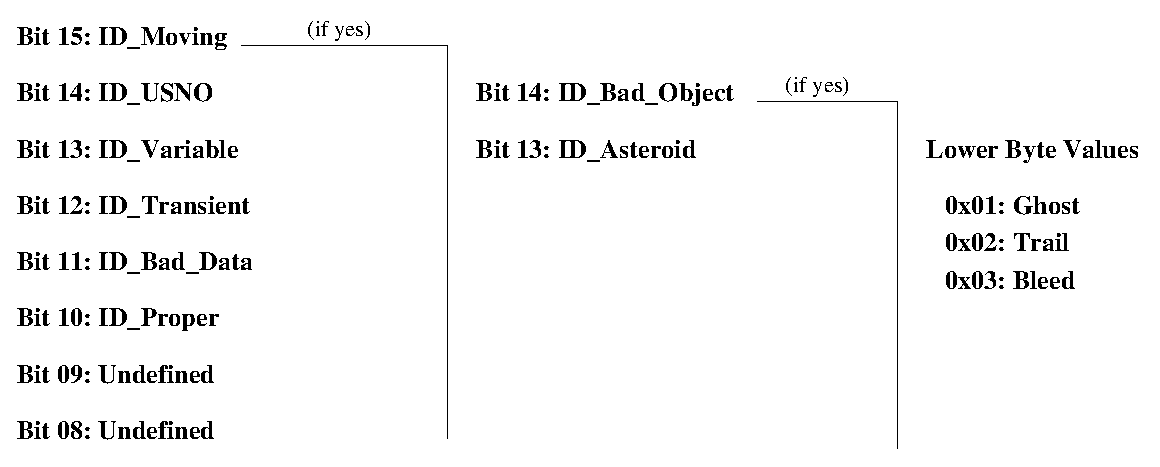
\psfig{file=flags.eps,width=9cm}
\caption{\label{flags} 
Pictoral representation of the Average.code flags.  The lower byte
value is used for specific definitions of object types.
}
\end{figure}

\subsection{Data Flags}

The identifications made by the above routines are noted as a set of
flags in the Average.code structure entry.  Some of these flags are
mutually exclusive, so a certain bit may have more than one meaning,
depending on the value of other bits.  Figure~\ref{flags} shows a
pictoral representation of the meaning of the different bit fields.
The uppermost bit (bit 15) determines if the object may be considered
a ``fixed'' star or something which has no fixed location.  If it is
not fixed, and this bit is 1, then there are several options.  The
second uppermost bit (bit 14) will be set if this object is one of the
three types of bad data flagged by {\tt markstar}.  The lower byte of
code is used to define the type of bad data: ghost, trail, or bleed.
Thus, any datapoints determined to be a satelite trail will have a
code value of 0xc002 (49154 decimal).  If an object is a moving
object, but not a bad datapoint, it may be identified as a ``rock''
(an asteroid) by the program {\tt markrock}.  In this case, the flag
for an asteroid is turned on (bit 13).  Thus anything identified as a
rock by {\tt markrock} will have a code value of 0xa000.  The lower
byte of code is not yet defined for asteroids, but could be reserved
for distinguishing different classes of asteroids (ie, on the basis of
orbital speeds, and so forth).  Objects which are fixed may have a
variety of possible flags.  First, an object may be identified with a
USNO star (bit 14).  It may be found to exhibit variability (bit 13),
implying that the relative photometry routine should ignore it.  If
may be a transient object (bit 12).  Note that, while an object
associated with a USNO object may not be transient, an object which is
variable may also not be associated with a USNO object.  Thus, we need
seperate bits for variable vs transient.  Different types of variable
objects may be represented with different values of the lower byte.
For example, a Cepheid may have a specific lower byte code of 0x01,
which an RR Lyra may have a lower byte code of 0x02.  Thus a Cepheid
associated with the USNO catalog would have a total code value of
0x6001. Finally, any of these types of non-moving objects may have
some bad individual measurements (bit 12) or may be found to have a
significant proper motion (bit 11).

\section{Holding it Together}

The preceeding sections describe the step-by-step analysis and
incorporation of the data from individual images.  However, the power
of the Pipeline comes in apply it to large numbers of images.  At
LONEOS, we are using four Pentinum II computers to analyse the roughly 200
images that are observed each night.  

It is best to think of the analysis of images occurring on groups of
images from a given night.  Of the set of processes discussed above,
those in section \ref{parallel} are performed on individual images
essentially independently of the other images.  The rest of the steps,
both the data incorporation ({\tt addstar} and the database cleaning
routines occur on the entire batch, one image at a time.  Thus, the
former routines can easily be run in parallel, but the latter routines
are run in serial to avoid having two programs writing to same part of
the database at the same time.  In this model, we would process all of
the images from a night through the parallel stage of the analysis and
then run the serial stage only after the entire night is finished in
the parallel stage.  We thus have a natural division of the pipeline
into two stages.  

The implementation of the two stages involves several programs, some
of which are specific to the LONEOS problem, and others which are more
general.  There are two layers of programs which enable batch
processing of many images and repeated batch processing over many
nights.  At the highest level, are Perl scripts which decide on a new
set of data.  At the next level down, these scripts call two main C
programs which run the images of a given night through the pipeline.  
A fixed set of files keeps a log of the nights and images that have
been processed, so the programs may know if a given night has already
been analysed. 

\subsection{lastnight}

The Perl script {\tt lastnight} looks at the disks used by the
observers to write the images from a given night.  Images are written
to a directory called /pallas/d[1-6]/NNNNNN where NNNNNN is an
abbreviation for the current night's date in the form YYMMDD (ie,
990223).  All of the images are stored in this directory with names
yyyyMMDDxxxxb.fits where yyyy is the full year, MM is month, DD is
date, and xxxx is a sequence number.  The 'b' refers to the 'b' CCD,
and the .fits extension is required.  The script {\tt lastnight} is
called by a cron job scheduled for 7am on {\tt hebe.lowell.edu}.  The
script searches the disks /pallas/d[1-6] for a directory of the right
form (basically any directory beginning with a number).  By default,
the program demands that the directory have a name of today's date,
but with the flag -any, it will accept any directory.  It then checks
to see if this directory have been already included in the
'processed.log' file.  If not, it lists all files with the right
ending (*b.fits) and places these names in a file.  It also writes the
name of the directory (along with some other data) in a file
'extracted.log'.  When it has successfully ended and identified some
data, it calls the next script, {\tt stage1} and then quits.  

\subsection{slurp}

An alternative to {\tt lastnight} is the Perl script {\tt slurp},
which looks for data on the tape archive.  This script looks at the
tape.log file and compares it to the file processed.log.  It tries to
identify nights listed in the tape.log which have not been included in
the processed.log.  If it finds any, it tries to download as much of
the data as will fit on the disk /pallas/d1.  This script is called
from within the {\tt stage1} script and is invoked if {\tt stage1} is
run without any data already in extracted.log.  

\subsection{stage1}

The Perl script {\tt stage1} takes the image list produced by {\tt
lastnight} or {\tt slurp} and passes the list to the controller
program {\tt control1} which performs the parallel analysis.  The
script has a few features to decide which files have been analysed
through the pipeline and to what extent.  If {\tt stage1} is called,
it should be able to figure out 1) if there is data ready to be
analysed, 2) if the data has been partially analysed, 3) which data
needs to be run through which part of the pipeline, and so forth.
These features are most useful if the analysis crashes in the middle
or needs to be restarted.  The {\tt stage1} script is meant to be run
without any arguments and it will figure out what needs to be done.
The one possible argument is the -once flag.  This flag tells {\tt
stage1} to analyse the data it finds and quit when it finishes, and
not call another instance of itself.  The script writes a log file
called \$scriptdir/stage1.NN.log where NN is a number in sequence
between all runs of {\tt stage1}.  A file stage1.count keeps track of
which number NN we are on.  When {\tt stage1} has finished the
analysis of a night's data, it writes the date in processed.log to
keep {\tt slurp} and {\tt lastnight} from re-running a night.

\subsection{stage2}
The serial stage processes are run by the Perl scrip {\tt stage2}.
Normally, this script is always running.  It waits for the name of a
night to be added to the processed.log file.  Once if finds a new name
in this file, it looks for the appropriate images in the file
YYMMDD.addlist.  It then submits the list to the second controlling
program {\tt control2}, which runs the images through {\tt addstar}.
Images which are successfully run through addstar have their *bf.fits
(flattened image) and *.obj (dophot output) files deleted.  When the
entire night is done, the rest of the *.obj and *bf.fits images are
deleted by {\tt stage2}, the directory with the *.cmp and *.log files
is tared and gzipped into the file YYMMNN.tgz.  The directory is then
deleted.  Finally, {\tt stage2} calls the script {\tt cleaning.pl}
which runs the cleanup programs ({\tt markstar - nrphot}) on the
database.  After a successful run, {\tt stage2} will automatically
respawn a new copy that waits until more data arrives.

\subsection{control1 / control2}
These two C-programs perform the tasks of farming the images out to
the different machines for analysis.  The two programs are essentially
identical, but {\tt control1} is allowed to use all machines and {\tt
control2} can only use one (hebe.lowell.edu, which has the database
local to it, mostly).  The two programs also run a different set of
program.  These controller programs start off by executing remote
shells (using ssh) on a list of machines.  These shells are then used
to execute the remote commands and are kept open the entire time the
process runs.  They maintain a list of images in a set of queues.  A
set of rules defines the order in which each image travels through the
queues.  Each queue is associated with a single process (flatten,
astrometry, etc).  Images which successfully run through a queue are
sent on to the defined 'next' queue, while images which fail are
instead sent to the defined 'fail' queue.  In most cases, the 'fail'
queue is a process which marks the image as bad and write the name in
a file, and then puts the image in the 'done' queue.  However, it is
possible for the 'fail' queue to be another attempt, such as in the
case of astrometry.  In this example, images which fail the default
astrometry are run through a second queue which tries again with the
-loneos flag set (this flag makes the assumption that the header
information about the LONEOS region number for the image is correct,
not the RA/DEC information).

The connections on the remote machines are handled as child processes
with communication through the stdin and stdout/stderr pipes.
Messages can be sent back and forth though these pipes, and messages
which are received from a process associated with an image are written
to a log file with the name imagename.log (where imagename is the root
name of the image).  The only required messages from the program are
messages saying ``SUCCESS'' or ``ERROR''.  The programs therefore all
end with either of these words.  The programs are started within the
controller as a command to the shell followed by and echo ``PROCESS
DONE''.  If the controller sees the message ``PROCESS DONE'' without
either ``SUCCESS'' or ``FAILURE'' (after waiting an appropriately long
time), it assumes the program crashed.  Currently, no timeout is
available for the programs.  The flat-field process is run in mana and
is a slightly special case.  We avoid re-loading the same flat many
times by starting a mana process once and running the flatten
procedures as mana function calls.  The images which are analysed
(with an indicator of success or failure at each stage) are written to
a file named YYMMDD.addlist by the {\tt control1} and YYMMDD.outlist
by {\tt control2}.

\section{Lock files}

A variety of locking mechanisms are used to avoid overwriting the
database or running more than one version of the controlling
programs.  there is a perl program, locks, which allows the user to
set or check the state of the different locks. 

\section{File locations}

\begin{verbatim}
database: /hebe/d27/database (also in /metis/d27/database as linked directories).
 lock files also go in this directory
workspace: /irene/d11/workspace - temporary storage of result files
dumpspace: /pallas/d1 - disk to store data dumped from the archive by slurp.
scriptdir: /metis/d11/logs - all log files
\end{verbatim}

\section{Visualization -- Status}

Visualization of the data in the photometry database can best be
performed with the program {\tt status}.  This is a command-line
driven program with a math and macro language which makes it easy to
perform complex tasks.  

First, a few notes about the user interface.  The interface has an
interaction similar to {\tt tcsh}.  The arrows allow editing of
previous commands.  You can also use emacs-like commands such as
cntl-a to reach the beginning of the line and cntl-e to reach the end.
There is command and file completion: if you type part of a command
(as the first thing on a line) and then type tab, it will fill in as
much as possible, until the word is not unique.  Typing tab twice at
that point will list the possible endings.  For any but the first word
on a line, the same thing will happen for the files in the current
directory.  It is also possible to type just a fraction of a command,
as long as it is unique.  An ambiguous command will list the possible
alternatives.  For example:
\begin{verbatim}
status: c
ambiguous command: c ( catalog cgrid clear create cursor )
\end{verbatim}

The shell is essentially an interpretive programming language.
Variables are set as follows:
\begin{verbatim}
status: $fred = 10
\end{verbatim}
Any expression within curly brackets \{\} is assumed
to be an arithmetical expression and is evaluated before the line is
executed.  For example:
\begin{verbatim}
echo {$fred*dcos(45)}
\end{verbatim}
would give the response 7.07107.  There are math functions cos, sin,
and tan, which operate on radian expressions, and also dcos, dsin,
dtan, which operate on degree expressions.  There are also the
equivalent inverse functions: eg., asin and dasin return radians and
degrees, respectively.  The help section on Math defines all of the
available math functions.  

\subsection{Miscellaneous Commands}
\begin{verbatim}
!                         -- system call
?                         -- list commands 
??                        -- list variables 
echo                      -- type this line 
exec                      -- system call
exit                      -- exit program 
help                      -- get help on a function 
output                    -- redirect output to file
quit                      -- exit program 
scan                      -- scan line from keyboard or file to variable 
wait                      -- wait until return is typed
which                     -- show command 
\end{verbatim}
Most of these are self-explanatory.  The command ?? prints the system
variables.  The {\tt help} command will provide help on a single
command or, without any arguments, will list all available help
files (this includes general help not associated with a specific
command).  

\subsection{Shell Programing}
\begin{verbatim}
break                     -- escape from function 
for                       -- loops 
if                        -- logical cases 
input                     -- read command lines from a file 
macro                     -- deal with the macros 
\end{verbatim}

There are several options for programming in {\tt status}.  First, a
file which contains a series of commands can be executed with {\tt
  input (filename)}.  It is also possible to define macros which will
behave much like regular commands.  A macro is defined by typing {\tt
  macro name} or {\tt macro create name} followed by the commands.
Arguments to the macro are assigned to the variables \$1 .. \$N and
the number of arguments is given by \$0.  Macros may be defined in
{\tt input} files, and in fact when {\tt status} is started, it loads
the file {\tt \~/.statusrc} which may contain default macros.  Simple
loops and if statements can be performed, and are quite useful for
complex macros.  

``If'' statements are similar in syntax to C if statements, but only
the following logical operators are available: $>$, $<$, $=$, !, $|$,
and \&.  Notice that (currently) there is no $>=$ or $<=$ symbol.  The
operator ! means ``not equal to'', but cannot be used to negate a
logical value.  The operators $|$ and \& have the meaning of ``or'' and
``and'' respectively.  Math expresions in the if statement must be
contained in curly braces, as elsewhere.  Variables with string values
may use the logical $=$ operator to test if two strings are the same.
``For'' loops are quite simplistic.  The form is:
\begin{verbatim}
for var first last delta
 (commands)
end
\end{verbatim}
The value of {\tt \$var} will start at the value {\tt first} and increment by
{\tt delta} after each loop.  The loop will stop after {\tt \$var} is greater
than {\tt stop}.  The value {\tt delta} is optional, with 1 assumed.
The value of {\tt \$var} may be changed during the loop, and if set
beyong the value of {\tt last} will end the loop early.  

\subsection{Vector Plotting}

\begin{verbatim}
box                       -- draw a box on the plot
clear                     -- erase plot
create                    -- create a new vector
cursor                    -- get coords from cursor
grid                      -- plot cartesian grid
hist                      -- create histogram from a vector
labels                    -- define labels for plot
limits                    -- define plot limits
plot                      -- plot a pair of vectors
print                     -- write vectors to file
ps                        -- define labels for plot
set                       -- vector math
style                     -- set the style for graph plots
vectors                   -- list vectors
zplot                     -- plot scaled points 
\end{verbatim}

In addition to scalar variables, {\tt status} can manipulate and
display 1-D vector variables.  Many of the commands which extract data
from the photometry database place the data in vectors as well as
plotting them.  A vector can also be created based on a number
sequence with the command {\tt create name Nelements start delta}.
The resulting vector has $Nelements$ entries, starting at a value of
$start$ and running until $start + delta*Nelements$.  If $delta$ is
0.0, all elements will have the value of $start$.  A histogram of a vector
may be made with the command {\tt hist}, which creates a new vector
containing the histogram of the first vector.  The data range and bin
size of the histogram are defined in same way as with create.  This
makes it easy to create the index vector that goes with a histogram
vector:  
\begin{verbatim}
hist y Ny 1 100 0.1
create dx 1 100 0.1
\end{verbatim}
The above will create a histogram of y in Ny and the index in dx.
Plotting this with {\tt plot dx Ny} will show the histogram.

Vector math is performed with a command of the form {\tt set new =
  (expression)}.  The expression is some math function employing
vectors and scalars.  A complete listing of the math operators
available in {\tt set} can be found in the help for {\tt set}.

Once vectors are defined, they may be plotted.  A pair of vectors can
be plotted against each other if they have the same number of entries.
The plotting is performed on the graphics window, Kapa.  There are
actually several graphics windows available to {\tt status}, any of
which may be used to plot at any time.  Some of the more complex
operations default to either graphics window 0 or 1, depending on the
context.  Except for those functions with a pre-defined window, all
plotting functions apply to the current graphics window unless an
option {\tt -n N} is given to specify a different window.  The
plotting style is determined by the command {\tt style} which can set
the line width, the line type (solid, dashed, dotted, etc), the point
type (box, cross, etc), the point size, the color, and whether a pair
of vectors is plotted as a sequence of points, a set of connected
lines, or a histogram.  Some functions which make plots use their own
styles, as discussed below.  The function {\tt limits} lets the user
set the range of the plot axes, or check the current setting.  The
command {\tt plot} will plot a pair of vectors on the current graphics
window using the current plotting style for that window.  The command
{\tt zplot} will plot a pair of vectors with the point size scaled by
a third vector, with maximum and minimum point sizes representing
specified values.  The {\tt cursor} command goes the other way: this
command puts the Kapa window in cursor mode and waits for input from
Kapa.  The user can then type any alphanumeric key on the graphics
windows and will be told both the pointer location (in the graphics
coordinates) and will have the coordinates stored in {\tt status}
variables.  For example, by typing ``1'' in the sky display window,
the RA and DEC of the pointer are stored in the variables {\tt \$R1}
and {\tt \$D1}.  This command can be used to let the user define
locations or regions of interest on the Kapa window. (Future addition:
{\tt button}, which does the same with the mouse buttons).  

\subsection{Database Functions}

\begin{verbatim}
gcat                        -- get catalog at location
gimages                     -- get images at location
gstar                       -- get star statistics
extract                     -- extract average vectors from catalogs
mextract                    -- extract measurement vectors from catalogs
imstats                    -- plot image statistics
imextract                   -- extract image vectors from database
lcat                        -- list catalogs in display region
cmatch                      -- match two catalogs
\end{verbatim}

There are a variety of other commands which directly refer to the
photometry database.  Some of these functions extract data of various
types from the database, others perform more complex plotting
operations.  The commands listed above are those which simply extract
data from the database.  The first three list information relevant to
a specific RA, DEC location on the sky: {\tt gcat (RA) (DEC)} lists
the catalog at the specified location and places the name in the
variable {\tt \$CATNAME}, {\tt gimages (RA) (DEC)} lists all images
which overlap the specified location, , {\tt gstars (RA) (DEC)
  (RADIUS)} lists data about the stars within a specified radius of
the specified location (all numbers above are given in decimal
degrees).  Similarly, {\tt lcat} lists the catalogs in the region.
Imstats lists statistics about each image

The next three commands extract a specific piece of information from
the photometry database and places it in a vector.  First, {\tt
  extract} will extract average values for each star and place it in a
vector.  Next, {\tt mextract} will extract measurement values for each
star and place it in a vector: as a result a single star may have
multiple entries in the measurement vectors.  Finally, {\tt imextract}
will extract image statistics into vectors (not yet implemented).


\begin{verbatim}
catalog                    -- plot catalog stars
cgrid                      -- plot sky coordinate grid
cplot                      -- plot vectors in sky coordinates
czplot                     -- plot scaled vectors in sky coordinates
images                     -- plot image boxes
imdense                    -- image density plot
lcurve                     -- plot lightcurve for a star
pcat                       -- plot catalog boundaries
region                     -- define sky region for plot
resid                      -- plot residuals
simage                     -- plot stars in an image
\end{verbatim}

There are two types of database plotting functions: those that display
or refer to the spatial charateristics of the data and those that
refer to other types of charatersitics, such as the time domain.  The
graphics window 0 is reserved for all plots of objects on the sky.
The command {\tt region} defines the current sky coordinates for plots
in graphic window 0.  The command {\tt pcat} plots the outline of all
photometry database files which are within the currently defined
region (and by default, only those with data).  {\tt images} plots the
outline of the images in the image database, while {\tt imdense} shows
the number of images at a location by randomly spacing dots within the
boundary of the images.  The command {\tt cgrid}
draws a grid in celestial coordinates on the for the current region.

The most complex, but also one of the most useful command is {\tt
  catalog}, which plots the positions of stars in the photometry
database (and others) on the sky.  There are many options to this
command.  One set allows the user to plot stars from the photometry
database (the default), from the HST GSC, or from an ASCII text file
with RA, DEC, and Mag in specified columns.  If the ASCII file has a
fixed number of bytes per line, the data can be more quickly loaded.
The size of the points may be scaled by the star magnitude, by the
number of observations of the star, or by the number of missing
datapoints for the star.  In addition, points may be plotted only if
they land in specified magnitude ranges, or with specified numbers of
measurements, or missed measurements.  Also, objects may be plotted
only if they have a specified Average.code, so that only asteroids or
only perfect stars may be plotted.  The plotted vectors may be saved,
if desired, and the source catalog epoch may be specified as different
from J2000 (only valid for ASCII data).

Several other commands relate to non-spatial charateristics of images
and stars.  {\tt lcurve} will plot a light curve for all stars within
some radius of a point.  {\tt resid} plots the photometry residuals
for a particular region file.  

\section{Some Examples}

\begin{figure}
\psfig{file=allsky.ps,width=16cm}
\caption{\label{allsky} 
Map of the entire sky, and images added to database.
}
\end{figure}

Fig.~\ref{allsky} shows a map of the entire sky, and the location
of the images currently in the database.  This picture was made with
the following commands: (output is not shown) \\
\begin{verbatim}
status: region 0 0 90 gls
status: cgrid
status: style -lw 2 -c red 
status: images
status: ps
\end{verbatim}
In this example, on the graphics window, the image boxes are shown in
red.  The user now has the possiblitiy of using the cursor command to
narrow in on a specific region, and so forth.  

\begin{figure}
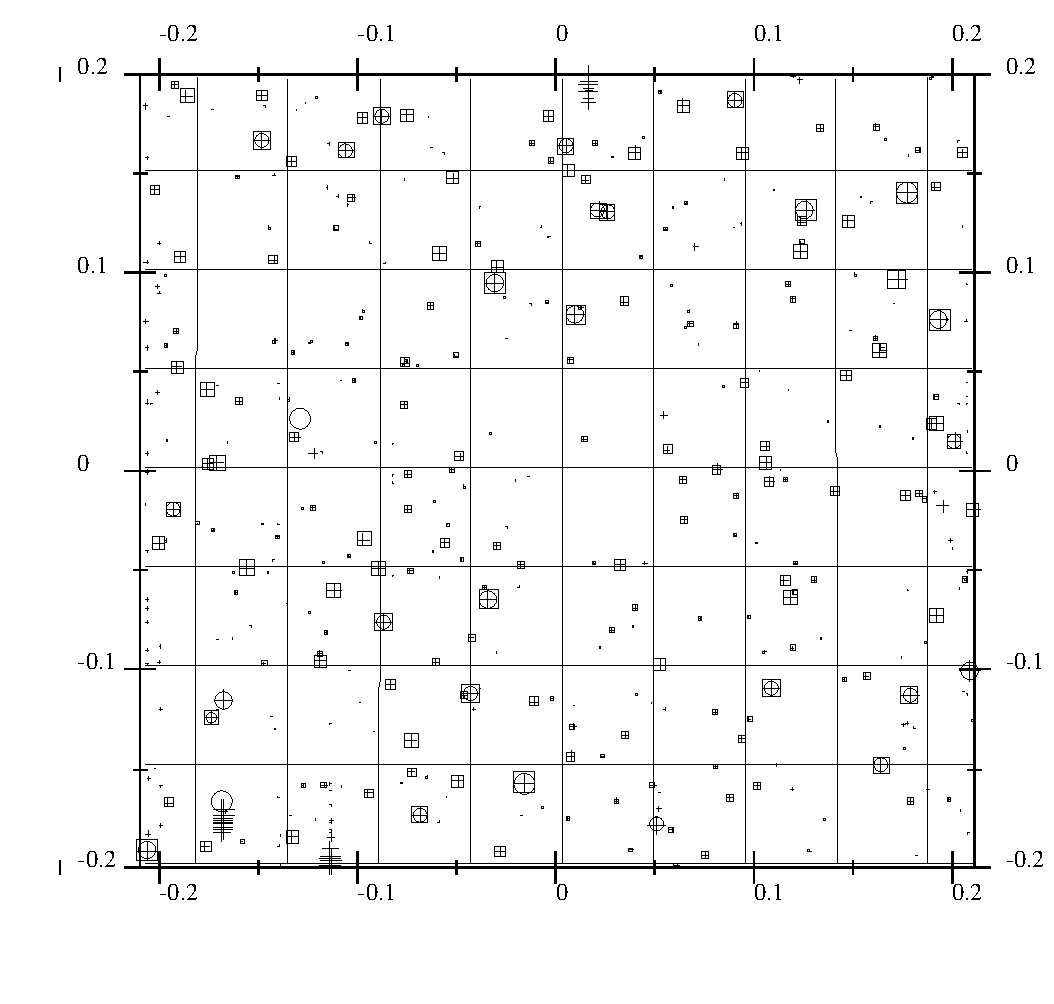
\psfig{file=catalog.ps,width=9cm}
\caption{\label{catalog} 
Comparison between HST GSC and photometry database astrometry. 
}
\end{figure}

Fig.~\ref{catalog} shows an example comparison of the photometry
database star positions and the HST Guide Star Catalog star
positions.  The crosses are from the photometry database while the
boxes are from the HST GSC.  The size of both points is a function of
brightness.  This plot was made with the following commands (starting
from the previous image):
\begin{verbatim}
status: cursor  (typed 1 on region of interest)
1 137.097858 22.698305
q 137.097858 22.698305
status: region $R1 $D1 0.5 TAN
status: cgrid
status: box
status: style -pt 0 
status: gcat $R1 $D1 
  0 n2230/1951.cpt *
status: catalog n2230/1951.cpt -m 12 18
status: style -pt 2
status: catalog n2230/1951.cpt -m 12 18 -g
\end{verbatim}

\begin{figure}
\psfig{file=lightcurve.ps,width=9cm}
\caption{\label{lightcurve} 
Lightcurve for several image stars.
}
\end{figure}

Fig.~\ref{lightcurve} shows an example lightcurve from three stars in
the above field.  The x axis shows the time in seconds, which the y
axis shows the star magnitudes.  This plot was made with the following commands (starting
from the previous image):
{\small
\begin{verbatim}
status: cursor
1 137.062562 22.791860
q 137.062562 22.791860
status: lcurve $R1 $D1 0.01 -l
status: box
status: gstar $R1 $D1 0.01
read 11318 stars from catalog file /host/pikake/d1/gene/loneos/allstars/n2230/1951.cpt (22462 total measurements)
508 /host/pikake/d1/gene/loneos/allstars/n2230/1951.cpt 137.068619 22.785400 18.438000  1 (2)  1.000000 1.000000
498 /host/pikake/d1/gene/loneos/allstars/n2230/1951.cpt 137.062820 22.792747 12.882000  3 (0)  1.000000 1.000000
501 /host/pikake/d1/gene/loneos/allstars/n2230/1951.cpt 137.064499 22.800817 15.480000  3 (0)  1.000000 1.000000
\end{verbatim}}
The last lines show the database information on the three stars.  

\section{Software Distribution}

\section{Programming Details}

\section {Comparison with USNO catalog}

I have made several comparisons between the USNO catalog and results
from running images from Loneos through the photometry pipeline.  In
general, there is a good agreement between the astrometry of the two
datasets.  There are specfic areas where the two disagree, however.
First, as discussed above, the USNO star positions may be
significantly different from the observed star positions simply
because of proper motion.  The first picure in the ``Comparisons
between Loneos + USNO'' pages shows several stars with significant
proper motion.  These are currently being flagged in the photometry
database as discussed.  Other differences evident in this first
picture include the classification of bright stars and the splitting
of faint and bright stars.  In the upper right of the image, two
bright stars are visible, one of which is actually a double.  The USNO
catalog does a good job of detecting both, but it also detects and
includes as stars several diffraction spike points.  The HST GSC only
detected a single point and did not split the star at all.  The Loneos
data in our pipeline did not detect the star at all due to saturation.
A star in the upper left corner shows the ability of {\tt dophot} in
the Loneos pipeline to split double stars.  This star is, on close
inspection, clearly a double.  The USNO catalog only detects one.  The
Pipeline not only splits the two stars, but it also makes the correct
cross-identification of the stars.  

The second set of pictures shows the ability of the Loneos pipeline to
deal with small galaxies.  There are two small galaxies in this field,
both of which are broken into 4 or 5 objects by the USNO catalog, but
maintained as single objects in the Loneos pipeline.  In another
example (not shown) a bright star within the disk of a small galaxies
was clearly split from the galaxy by the pipeline (and also by USNO).

\appendix
\section{Parameter file params.txt}
\begin{verbatim}
# Configuration file for Loneos analysis pipeline

# important files and directories
GSCFILE                 /host/pikake/d1/gene/gsc/GSCregions.tbl
GSC_DIR                 /host/pikake/d1/gene/gsc
CATDIR                  /host/radon/rad3/gene/photcat2
IMAGE_CATALOG           /host/radon/rad3/gene/photcat2/Images.dat
IMAGE_CATALOG_TEMPLATE  /host/radon/rad3/gene/photcat2/template.cat
CATALOG_TEMPLATE        /host/radon/rad3/gene/photcat2/template.cat
ROCK_CATALOG            /host/radon/rad3/gene/photcat2/Rocks.dat
USNO_CDROM              /host/tycho/mnt/md0/kevin/zones
LONEOS_REGIONS          /host/pikake/h1/gene/loneos3/regions.map

# parameters for "fstat"
# instrumental mag zero point
ZERO_PT                 24.5
DOPHOT_CHAR_LINE        129
DOPHOT_TYPE_FIELD       5
DOPHOT_AP_FIELD         91
DOPHOT_PSF_FIELD        52
MIN_SN_FSTAT            6.0

# parameters for "gastro"
DEFAULT_RADIUS   32.0
MINIMUM_RADIUS   1.5
MIN_ERROR        0.6
MIN_PRECISE      0.12
CCD_PC1_1        1
CCD_PC2_2        -1    # for loneos
CCD_PC1_2        0
CCD_PC2_1        0
ASEC_PIX         2.82
NFIELD           3.0
MMIN             6.0
ROT_ZERO         0
dROT             1.0
NROT             2
POLAR_AXIS_RA    -90.0
POLAR_AXIS_DEC   89.88
RA_OFFSET        -90.0
DEC_OFFSET        0.0

# parameters for "addstar"
# airmass extinction coefficient (in mag / airmass)
NSIGMA                  3.0
ALPHA                   0.1
XOVERSCAN               60
YOVERSCAN               50

# parameters for "controller"
IN_DIR                  /host/pikake/h1/gene
OUT_DIR                 /host/pikake/h1/gene/loneos4/
DOPHOT_PARAMS           /host/pikake/h1/gene/src/ohana/config/default_parameters
FLATTEN_SCRIPT          /host/pikake/h1/gene/src/ohana/config/test.pro
NEW_IMAGES              images.dat
USERNAME                gene
PASSWORD                gene

# here we list all available machines
NMACHINES               2
MACHINE0                pikake.astro.washington.edu
MACHINE1                mildew.astro.washington.edu

# here we define which machines which are always free
fMACHINE0               1
fMACHINE1               0

# here we define the machine which runs the database 
LOCAL_MACHINE           0

# parameters for "status"
TIME_REFERENCE          90/01/01 00:00:00

# parameters for "nrphot"
# make this one small to boost change of getting an early region 
TAU                     3.0             
SCATTER_LIM             15.0
MAG_LIM                 17.0
IMAGE_SCATTER           0.075
NIMAGE_SCATTER          1.5
STAR_SCATTER            0.05

### parameters for "markstar"
SEARCH_RADIUS           360   # region for initial trail hunt, in arcsec 
TRAIL_WIDTH             5.0   # expected trail width, in arcsec
NANGLE_BINS             180   # Number of angular bins in 180 degrees
NPTSINLINE              5     # minimum points needed for trail
MIN_DENSITY             0.025 # minimum linear density in star/arcsec
SPACE_SIGMA             10.0  # how much denser than average for trail?
# parameters defining bright star exclusion regions
BRIGHT_XTRAIL_WIDTH       5.0 # faintest sat. star
BRIGHT_XTRAIL_MAG         9.5 # faintest sat. star
BRIGHT_XTRAIL_SLOPE     -80.0 # exclusion radius = BRIGHT_SLOPE * (mag - BRIGHT_MAG)
BRIGHT_YTRAIL_WIDTH       5.0 # faintest sat. star
BRIGHT_YTRAIL_MAG        11.0 # faintest sat. star
BRIGHT_YTRAIL_SLOPE    -400.0 # exclusion radius = BRIGHT_SLOPE * (mag - BRIGHT_MAG)
BRIGHT_HALO_MAG           8.5 # faintest sat. star
BRIGHT_HALO_SLOPE       -28.0 # exclusion radius = BRIGHT_SLOPE * (mag - BRIGHT_MAG)
# parameters which define the ghosts
GHOST_MAG               7.5
GHOST_RADIUS            200   # in arcsec
OPTICAL_AXIS1           2154.0
OPTICAL_AXIS2           2193.0

# parameters for "addusno"
USNO_RADIUS             5.0   # in arcsec
USNO_PROPER             20.0   # in arcsec
USNO_RED                1000  # code for USNO Red data
USNO_BLUE               1001  # code for USNO Blue data
# /mnt/cdrom

# parameters for "markrock"
ROCK_RADIUS             2.0   # in arcsec
ROCK_MAX_RADIUS         20.0  # in arcsec
ROCK_MAX_SPEED          0.1   # in arcsec / sec
\end{verbatim}

\end{document}
